\section{Durchführung}
\label{sec:Durchführung}
Die Versuchsanordnung ist in Abb. \ref{fig:Anordnung} abgebildet.
\begin{figure}
    \centering
    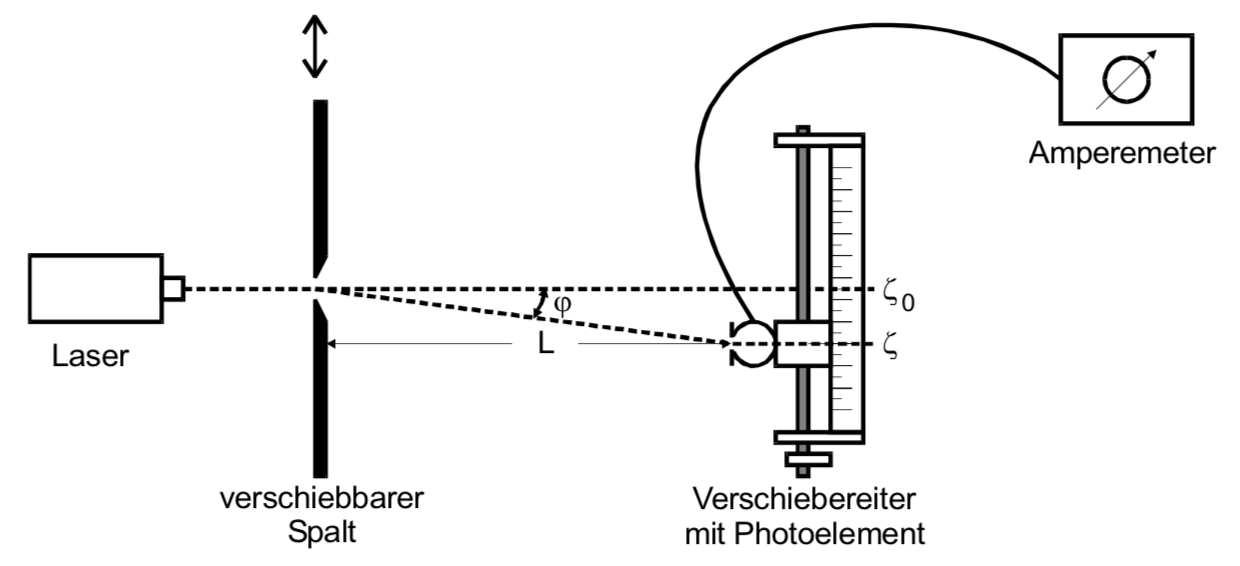
\includegraphics[width=12cm, height=6cm]{build/Anordnung.png}
    \caption{Versuchsanordnung zur Messung der Stromstärke des
    Beugungsbildes verschiedener Spalte. \cite{V406}}
    \label{fig:Anordnung}
\end{figure}

\noindent Zunächst wird der Abstand des Spaltes zum Detektor gemessen.
Anschließend wird der Off-Strom der Diode gemessen, wobei
der Laser ausgeschaltet und eine Ableselampe eingeschaltet ist.
\newline
Die Apparatur wird so ausgerichtet, dass das Hauptmaximum des 
Beugungsbildes auf dem Detektorspalt liegt.
\newline
Das Beugungsbild des ersten Einzelspaltes wird punktweise
mit einer Schrittweite von $\SI{0.5}{\milli\meter}$ ausgemessen.
Dazu wird die Stromstärke an einem Amperemeter abgelesen.
\newline
Für den zweiten Einzelspalt wird dasselbe wiederholt.
\newline
Die Messung des Beugungsbildes des Doppelspalts wird ebenfalls
punktweise mit einer Schrittweite von $\SI{0.25}{\milli\meter}$ 
durchgeführt.